% Created 2017-02-01 Wed 03:12
\documentclass[11pt]{article}
\usepackage[utf8]{inputenc}
\usepackage[T1]{fontenc}
\usepackage{fixltx2e}
\usepackage{graphicx}
\usepackage{longtable}
\usepackage{float}
\usepackage{wrapfig}
\usepackage{rotating}
\usepackage[normalem]{ulem}
\usepackage{amsmath}
\usepackage{textcomp}
\usepackage{marvosym}
\usepackage{wasysym}
\usepackage{amssymb}
\usepackage{hyperref}
\tolerance=1000
\usepackage[margin=0.75in]{geometry} \usepackage{graphicx}
\author{Anthony Tam, 1002583402}
\date{\today}
\title{CSC258 Prelab Four}
\hypersetup{
  pdfkeywords={},
  pdfsubject={},
  pdfcreator={Emacs 26.0.50.1 (Org mode 8.2.10)}}
\begin{document}

\maketitle


\section{SR Latch Truth Table}
\label{sec-1}

\begin{center}
\begin{tabular}{rrrrr}
C & S & R & Q & Q'\\
\hline
0 & X & X & X & X\\
1 & 0 & 0 & X & X\\
1 & 0 & 1 & 0 & 1\\
1 & 1 & 0 & 1 & 0\\
1 & 1 & 1 & 0 & 0\\
\end{tabular}
\end{center}

Notes:
\begin{itemize}
\item The clock does not play a major role in the truth table
\begin{itemize}
\item When the clock is 0, we are always in a latch state and retain the previous value (Denoted by X)
\end{itemize}
\end{itemize}

\section{Diagram of a D latch}
\label{sec-2}
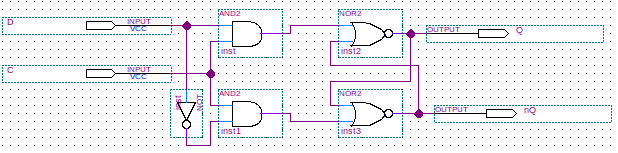
\includegraphics[width=\textwidth]{dlatch.png}

\section{Diagram of a D Flip Flop}
\label{sec-3}
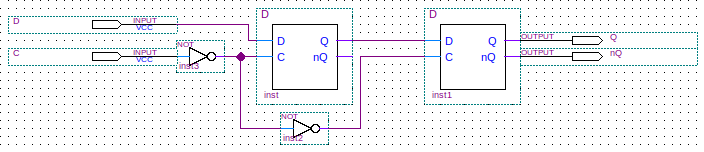
\includegraphics[width=\textwidth]{dflipflop.png}
% Emacs 26.0.50.1 (Org mode 8.2.10)
\end{document}
